\documentclass[sigplan,screen]{acmart} 
%
\usepackage[utf8]{inputenc}
\usepackage[british]{babel}
\usepackage{hyperref}
%\usepackage[left=0.5in, right=0.5in, top=1in, bottom=1in]{geometry}
\usepackage{graphicx}
\usepackage{listings}
\usepackage{xcolor}
\usepackage{amsmath,amssymb,amsthm}
\usepackage{fancyhdr}
\usepackage{extramarks}
\usepackage{enumerate}
\usepackage{subcaption}
\usepackage{caption}
\usepackage{float}
\usepackage{stmaryrd}
\usepackage{amstext}
\usepackage{mathtools}
\usepackage{multicol}
\usepackage{url}
\usepackage{hyperref}
\usepackage{array}

% References
\newcommand\pepm{\cite{10.1145/3441296.3441393}}
\newcommand\cornell{\cite{10.1145/358746.358755}}
\newcommand\hazel{\cite{conf/popl/Hazelnut17}}
\newcommand\scratch{\cite{10.1145/1592761.1592779}}
\newcommand\alice{\cite{10.1145/332040.332481}}
\newcommand\elmcore{\cite{Elm-lang-core}}
\newcommand\elmsvg{\cite{Elm-lang-svg}}
\newcommand\elmmat{\cite{Elm-lang-material}}
\newcommand\elmhtml{\cite{Elm-lang-html}}

% Metadata
\newcommand\mdtitle{Implementation of a Type-Safe Structure Editor}
\newcommand\mdtitleshort{Implementation of a Type-Safe Structure Editor}
\newcommand\mdauthor{
  Nicolaj Richs-Jensen \\
  \url{vzq239@alumni.ku.dk}
  \and
  Thorbjørn Bülow Bringgaard \\
  \url{vwc415@alumni.ku.dk}
  \and
  Tórur Feilberg Zachariasen \\
  \url{xsz482@alumni.ku.dk}
}
\newcommand\mdauthorshort{Nicolaj, Thorbjørn, Tórur \& Hans}
\newcommand\mddate{\today}

% Syntax
\newcommand\app[2]{#1~#2}
\newcommand\abs[2]{\lambda #1.#2}
\newcommand\cursor[1]{\llbracket #1 \rrbracket}
\newcommand\breakpoint[1]{\langle #1 \rangle}
\newcommand\hole{\llparenthesis\rrparenthesis}
\newcommand\transition[1]{\xrightarrow[]{\text{#1}}}

\newcommand\AST{\textbf{Ast}}
\newcommand\Ast{%
  a &::= x
  \mid c
  \mid \app{a_1}{a_2}
  \mid \abs{x}{a}
  \mid \cursor{a}
  \mid \breakpoint{a}
  \mid \hole
}

% Cursor contexts
\newcommand{\cursorhole}{\[\cdot\]}
\newcommand{\Cts}{C &::= [\cdot] \mid \app{C}{\hat{a}} \mid \app{\hat{a}}{C} \mid \abs{x}{C} \mid \breakpoint{C}}

\newcommand\aHat{%
  \hat{a} &::= x
  \mid c
  \mid \app{\hat{a}_1}{\hat{a}_2}
  \mid \abs{x}{\hat{a}}
  \mid \breakpoint{\hat{a}}
  \mid \hole
}

\newcommand\aDot{%
  \dot{a} &::= \cursor{\hat{a}}
  \mid \abs{x}{\cursor{\hat{a}}}
  \mid \app{\cursor{\hat{a}_1}}{\hat{a}_2}
  \mid \app{\hat{a}_1}{\cursor{\hat{a}_2}}
  \mid \breakpoint{\cursor{\hat{a}}}
}

% Editor expressions
\newcommand\pre[2]{#1.#2}
\newcommand\bicond[3]{\ensuremath{#1 \Rightarrow #2 \mid #3}}
\newcommand\seqcomp[2]{\ensuremath{#1 \ggg #2}}
\newcommand\rec[2]{\ensuremath{\texttt{rec}~#1.#2}}
\newcommand\call[1]{#1}
\newcommand\nil{\mathbf{0}}
\newcommand\Exp[2]{\breakpoint{#1,\, #2}}

\newcommand\edt{\textbf{Edt}}
\newcommand\Edt{%
  E &::= \pre{\pi}{E}
  \mid \bicond{\phi}{E_1}{E_2}
  \mid \seqcomp{E_1}{E_2}
  \mid \rec{x}{E}
  \mid \call{x}
  \mid \nil
}

% Prefix commands
\newcommand\eval{\texttt{eval}}
\newcommand\sub[1]{\ensuremath{\{ #1 \}}}
\newcommand\child[1]{\ensuremath{\texttt{child}~#1}}
\newcommand\parent{\texttt{parent}}

\newcommand\aep{\textbf{Aep}}
\newcommand\Aep{%
  \pi &::= \eval
  \mid \sub{D}
  \mid \child{n}
  \mid \parent
}

% AST node modifiers
\newcommand\var[1]{\texttt{var}~x}
\newcommand\const[1]{\texttt{const}~c}
\newcommand\aamApp{\texttt{app}}
\newcommand\aamLambda[1]{\texttt{lambda}~#1}
\newcommand\aamBreak{\texttt{break}}
\newcommand\aamHole{\texttt{hole}}

\newcommand\aam{\textbf{Aam}}
\newcommand\Aam{%
  D &::= \var{x}
  \mid \const{c}
  \mid \aamApp
  \mid \aamLambda{x}
  \mid \aamBreak
  \mid \aamHole
}

% Conditions
\newcommand\conjunction[2]{#1 \land #2}
\newcommand\disjunction[2]{#1 \lor #2}
\newcommand\at[1]{@#1}
\newcommand\possibly[1]{\Diamond #1}
\newcommand\necessarily[1]{\Box #1}

\newcommand\eed{\textbf{Eed}}
\newcommand\Eed{%
  \phi &::= \neg\phi
  \mid \conjunction{\phi_1}{\phi_2}
  \mid \disjunction{\phi_1}{\phi_2}
  \mid \at{D}
  \mid \possibly{D}
  \mid \necessarily{D}
}

% Reduction rules
%% Table 1
\newcommand\CondOne{%
  \frac{a \vDash \phi}
  {\Exp{\bicond{\phi}{E_1}{E_2}}{a}\transition{$\epsilon$}\Exp{E_1}{a}}
}

\newcommand\CondTwo{%
  \frac{a \nvDash \phi}
  {\Exp{\bicond{\phi}{E_1}{E_2}}{a}\transition{$\epsilon$}\Exp{E_2}{a}}
}

\newcommand\Eval{%
  \frac{a \to v}
  {\Exp{\pre{\eval}{E}}{a}\transition{$v$}\Exp{E}{a}}
}

\newcommand\Seq{%
  \frac{\Exp{E_1}{a}\transition{$\alpha$}\Exp{E_1'}{a'}}
  {\Exp{\seqcomp{E_1}{E_2}}{a}\transition{$\alpha$}\Exp{\seqcomp{E_1'}{E_2}}{a'}}
}

\newcommand\Struct{%
  \frac{E_1 \equiv E_2\quad\Exp{E_2}{a}\transition{$\alpha$}\Exp{E_2'}{a'} \quad E_2' \equiv E_1'}
  {\Exp{E_1}{a}\transition{$\alpha$}\Exp{E_1'}{a'}}
}

\newcommand\Context{%
  \begin{aligned}
     & \frac{a \transition{$\pi$} a'}
    {\Exp{\pre{\pi}{E}}{C[a]}\transition{$\pi$}\Exp{E}{C[a']}} \\
     & \text{where } \pi \neq \eval
  \end{aligned}
}

%% Table 2
\newcommand\Var{%
  \frac{}
  {\cursor{\hat{a}}\transition{\{var x\}}\cursor{x}}
}

\newcommand\Hole{%
  \frac{}
  {\cursor{\hat{a}}\transition{\{hole\}}\cursor{\hole}}
}

\newcommand\Const{%
  \frac{}
  {\cursor{\hat{a}}\transition{\{const c\}}\cursor{c}}
}

\newcommand\App{%
  \frac{}
  {\cursor{\hat{a}}\transition{\{app\}}\cursor{\app{\hole}{\hole}}}
}

\newcommand\BreakOne{%
  \frac{\hat{a} \neq \breakpoint{\hat{a}'}}
  {\cursor{\hat{a}}\transition{\{break\}}\cursor{\breakpoint{\hat{a}}}}
}

\newcommand\BreakTwo{%
  \frac{}
  {\cursor{\breakpoint{\hat{a}}}\transition{\{break\}}\cursor{\hat{a}}}
}

\newcommand\LAMBDA{%
  \frac{}
  {\cursor{\hat{a}}\transition{\{lambda x\}}\cursor{\abs{x}{\hole}}}
}

%% Table 3
\newcommand\AppCOne{%
  \frac{}
  {\cursor{\app{\hat{a}_1}{\hat{a}_2}}\transition{child 1}\app{\cursor{\hat{a}_1}}{\hat{a}_2}}
}

\newcommand\AppCTwo{%
  \frac{}
  {\cursor{\app{\hat{a}_1}{\hat{a}_2}}\transition{child 2}\app{\hat{a}_1}{\cursor{\hat{a}_2}}}
}

\newcommand\AppPOne{%
  \frac{}
  {\app{\cursor{\hat{a}_1}}{\hat{a}_2}\transition{parent}\cursor{\app{\hat{a}_1}{\hat{a}_2}}}
}

\newcommand\AppPTwo{%
  \frac{}
  {\app{\hat{a}_1}{\cursor{\hat{a}_2}}\transition{parent}\cursor{\app{\hat{a}_1}{\hat{a}_2}}}
}

\newcommand\ABSC{%
  \frac{}
  {\cursor{\abs{x}{\hat{a}}}\transition{child 1}\abs{x}{\cursor{\hat{a}}}}
}

\newcommand\ABSP{%
  \frac{}
  {\abs{x}{\cursor{\hat{a}}}\transition{parent}\cursor{\abs{x}{\hat{a}}}}
}

\newcommand\BreakC{%
  \frac{}
  {\cursor{\breakpoint{\hat{a}}}\transition{child 1}\breakpoint{\cursor{\hat{a}}}}
}

\newcommand\BreakP{%
  \frac{}
  {\breakpoint{\cursor{\hat{a}}}\transition{parent}\cursor{\breakpoint{\hat{a}}}}
}

%% Table 4
\newcommand\AtVar{%
  \frac{}
  {x \vDash \at{(\text{var }y)}}
}

\newcommand\AtConst{%
  \frac{}
  {c \vDash \at{(\text{const }c)}}
}

\newcommand\AtHole{%
  \frac{}
  {\hole \vDash \at{\text{hole}}}
}

\newcommand\AtApp{%
  \frac{}
  {\app{\hat{a}_1}{\hat{a}_2} \vDash \at{\text{app}}}
}

\newcommand\AtAbs{%
  \frac{}
  {\abs{x}{\hat{a}} \vDash \at{\text{lambda }y}}
}

\newcommand\AtBreak{%
  \frac{}
  {\breakpoint{\hat{a}} \vDash \at{\text{break}}}
}

%% Table 5
\newcommand\PosTrivial{%
  \frac{\hat{a} \vDash \at{D}}
  {\hat{a} \vDash \possibly{D}}
}

\newcommand\PosAppOne{%
  \frac{\hat{a}_1 \vDash \possibly{D}}
  {\app{\hat{a}_1}{\hat{a}_2} \vDash \possibly{D}}
}

\newcommand\PosAppTwo{%
  \frac{\hat{a}_2 \vDash \possibly{D}}
  {\app{\hat{a}_1}{\hat{a}_2} \vDash \possibly{D}}
}

\newcommand\PosAbs{%
  \frac{\hat{a} \vDash \possibly{D}}
  {\abs{x}{\hat{a}} \vDash \possibly{D}}
}

\newcommand\PosBreak{%
  \frac{\hat{a} \vDash \possibly{D}}
  {\breakpoint{\hat{a}} \vDash \possibly{D}}
}

\newcommand\NecTrivial{%
  \frac{\hat{a} \vDash \at{D}}
  {\hat{a} \vDash \necessarily{D}}
}

\newcommand\NecApp{%
  \frac{\hat{a}_1 \vDash \possibly{D}\quad\hat{a}_2 \vDash \possibly{D}}
  {\app{\hat{a}_1}{\hat{a}_2} \vDash \necessarily{D}}
}

\newcommand\NecAbs{%
  \frac{\hat{a} \vDash \possibly{D}}
  {\abs{x}{\hat{a}} \vDash \necessarily{D}}
}

\newcommand\NecBreak{%
  \frac{\hat{a} \vDash \possibly{D}}
  {\breakpoint{\hat{a}} \vDash \necessarily{D}}
}


%% Table 6
\newcommand\BConst{%
  \frac{}
  {c \to c}
}

\newcommand\BAbs{%
  \frac{}
  {\abs{x}{a}\to\abs{x}{a}}
}

\newcommand\BCursor{%
  \frac{a \to v}
  {\cursor{a} \to v}
}

\newcommand\BApp{%
  \begin{aligned}
     & \frac{a_1 \to \abs{x}{a_1'} \quad a_2 \to v \quad a_1'\{v/x\} \to v'}
    {\app{a_1}{a_2} \to v'}                                                  \\
     & \text{where } v \notin \textbf{BVal} \cup \textbf{HVal}
  \end{aligned}
}

\newcommand\BAppBOne{%
  \frac{a_1 \to w}
  {\app{a_1}{a_2} \to \app{w}{a_2}}
}

\newcommand\BAppBTwo{%
  \frac{a_1 \to \abs{x}{a_1'} \quad a_2 \to w}
  {\app{a_1}{a_2} \to \app{\abs{x}{a_1'}}{w}}
}

\newcommand\BAppHOne{%
  \frac{a_1 \to u \quad a_2 \to v}
  {\app{a_1}{a_2} \to \app{u}{v}}
}

\newcommand\BAppHTwo{%
  \frac{a_1 \to \abs{x}{a_1'} \quad a_2 \to u}
  {\app{a_1}{a_2} \to \app{\abs{x}{a_1'}}{u}}
}

\newcommand\BBreakB{%
  \frac{}
  {\breakpoint{a}\to\breakpoint{a}}
}


% Values
\newcommand\val{\textbf{Val}}
\newcommand\Val{%
  v &::= c
  \mid \abs{x}{a}
  \mid w
  \mid u
}

\newcommand\hval{\textbf{HVal}}
\newcommand\HVal{%
  u &::= \hole
  \mid \app{u}{v}
  \mid \app{\abs{x}{a}}{u}
}

\newcommand\bval{\textbf{BVal}}
\newcommand\BVal{%
  w &::= \breakpoint{a}
  \mid \app{w}{a}
  \mid \app{\abs{x}{a}}{w}
}


% Types
\newcommand\pth{\textbf{Pth}}
\newcommand\Pth{p ::= p~T \mid \epsilon}
\newcommand\atyp{\textbf{ATyp}}
\newcommand\Atyp{%
  \tau ::= b
  \mid \tau_1 \to \tau_2
  \mid \breakpoint{\tau}
  \mid ~?
}
\newcommand\ctyp{\textbf{CTyp}}
\newcommand\Ctyp{T ::= \texttt{one} \mid \texttt{two}}
\newcommand\actx{\textbf{ACtx}}
\newcommand\ectx{\textbf{ECtx}}
\newcommand\elm[1]{\texttt{#1}}
\newcommand\typ[1]{\textbf{#1}}
\newcommand\ctx[1]{\Gamma_{#1}}
\newcommand\bind[2]{#1 : #2}

% Type rules
%% AST type rules
\newcommand\TConfiguration{%
  \frac{\emptyset \vdash \bind{a}{\tau} \quad p,\ctx{e} \vdash \bind{E}{ok}}
  {p,\ctx{e} \vdash \bind{\breakpoint{E,a}}{ok}}\\
}
\newcommand\TVar{%
  \frac{\ctx{a}(x) = \tau}
  {\ctx{a} \vdash \bind{x}{\tau}}
}

\newcommand\TConst{%
  \frac{}
  {\ctx{a} \vdash \bind{c}{b}}
}

\newcommand\TCursor{%
  \frac{\ctx{a} \vdash \bind{a}{\tau}}
  {\ctx{a} \vdash \bind{\cursor{a}}{\tau}}
}

\newcommand\TLambda{%
  \frac{\ctx{a},~\bind{x}{\tau_1} \vdash \bind{a}{\tau_2}}
  {\ctx{a} \vdash \abs{\bind{x}{\tau_1}}{\bind{a}{\tau_1\to\tau_2}}}
}

\newcommand\TBreak{%
  \frac{\ctx{a} \vdash \bind{a}{\tau}}
  {\ctx{a} \vdash \bind{\breakpoint{a}}{\breakpoint{\tau}}}
}

\newcommand\THole{%
  \frac{}
  {\ctx{a} \vdash \bind{(\bind{\hole}{\tau})}{\tau}}
}

\newcommand\TApp{%
  \frac{\ctx{a} \vdash \bind{a_1}{\tau_3} \quad \tau_3\sim\tau_1\to\tau_2 \quad \ctx{a} \vdash \bind{a_2}{\tau_1}}
  {\ctx{a} \vdash \bind{\app{a_1}{a_2}}{\tau_2}}
}

%% Edt type rules
\newcommand\TEval{%
  \frac{p,\ctx{e} \vdash \bind{E}{ok}}
  {p,\ctx{e} \vdash \bind{\pre{\eval}{E}}{ok}}
}

\newcommand\TRef{%
  \frac{}
  {p,\ctx{e} \vdash \bind{x}{ok}}
}

\newcommand\TNil{%
  \frac{}
  {p,\ctx{e} \vdash \bind{\nil}{ok}}
}

\newcommand\TChOne{%
  \frac{\ctx{e}(p~\texttt{one}) = (\ctx{a}, \tau) \quad p~\texttt{one}, \ctx{e} \vdash \bind{E}{ok}}
  {p, \ctx{e} \vdash \bind{\pre{(\child 1)}{E}}{ok}}
}

\newcommand\TChTwo{%
  \frac{\ctx{e}(p~\texttt{two}) = (\ctx{a}, \tau) \quad p~\texttt{two}, \ctx{e} \vdash \bind{E}{ok}}
  {p, \ctx{e} \vdash \bind{\pre{(\child 2)}{E}}{ok}}
}

\newcommand\TParent{%
  \frac{\ctx{e}(p) = (\ctx{a}, \tau) \quad p, \ctx{e} \vdash \bind{E}{ok}}
  {p~T, \ctx{e} \vdash \bind{\pre{\parent}{E}}{ok}}
}

\newcommand\TSeq{%
  \begin{aligned}
    & \frac{p,p'~\ctx{e} \vdash \bind{E_1}{ok} \quad p',\bar{p'}~\ctx{e} \vdash \bind{E_2}{ok}}
    {p,\ctx{e} \vdash \bind{\seqcomp{E_1}{E_2}}{ok}} \\
    & \text{for } p' = path(p,E_1)
  \end{aligned}
}

\newcommand\TRec{%
  \begin{aligned}
  & \frac{\ctx{e}(p) = (\ctx{a},\tau) \quad p,(\emptyset,\bind{p}{(\emptyset,?)}) \vdash \bind{E}{ok}}
  {p, \ctx{e} \vdash \bind{\rec{x}{E}}{ok}} \\
  & \text{if } path(p,E)=p
  \end{aligned}
}

\newcommand\TCond{%
  \begin{aligned}
  & \frac{p, update(\ctx{e},\delta \cup \{ (p, (\ctx{a}, \tau))\}) \vdash \bind{E_1}{ok} \quad p, \ctx{e} \vdash \bind{E_2}{ok}}
  {p, \ctx{e} \vdash \bind{\bicond{\phi}{E_1}{E_2}}{ok}}\\
  & \text{if~~~~} path(p,E_1) = path(p,E_2)\\
  & \text{and } (\ctx{a},\tau) = types(\phi, (\emptyset,?))\\
  & \text{and } \delta = \cap_{D \in limits(\phi,\aam)} follows(D,p)
  \end{aligned}
}

\newcommand\TSubVar{%
  \frac{\ctx{e}(p) = (\ctx{a}, \tau) \quad \ctx{a}(x) = \tau' \quad \tau \sim \tau' \quad p,(\bar{p}~\ctx{e}, \bind{p}{(\ctx{a},\tau')}) \vdash \bind{E}{ok}}
  {p, \ctx{e} \vdash \bind{\pre{\{\var x\}}{E}}{ok}}
}

\newcommand\TSubHole{%
  \frac{\ctx{e}(p) = (\ctx{a},\tau') \quad \tau \sim \tau' \quad p,(\bar{p}~\ctx{e},\bind{p}{(\ctx{a},\tau)}) \vdash \bind{E}{ok}}
  {p, \ctx{e} \vdash \bind{\pre{\{\bind{\texttt{hole}}{\tau}\}}{E}}{ok}}
}

\newcommand\TSubConst{%
  \frac{\ctx{e}(p)=(\ctx{a},\tau) \quad \tau \sim b \quad p, (\bar{p}~\ctx{e},\bind{p}{(\ctx{a},b)}) \vdash \bind{E}{ok}}
  {p, \ctx{e} \vdash \bind{\pre{\{\const c\}}{E}}{ok}}
}

\newcommand\TSubApp{%
  \begin{aligned}
  & \frac{\ctx{e}(p) = (\ctx{a},\tau_2') \quad \tau_2 \sim \tau_2' \quad p,\ctx{e}' \vdash \bind{E}{ok}}
  {p, \ctx{e} \vdash \bind{\pre{\{\bind{\texttt{app}}{\tau_1\to\tau_2,\tau_1}\}}{E}}{ok}}\\
  & \text{where } \ctx{e}' = \bar{p}~\ctx{e},\bind{p}{(\ctx{a},\tau_2)},\bind{p~\texttt{one}}{(\ctx{a},\tau_1\to\tau_2)},\bind{p~\texttt{two}}{(\ctx{a},\tau_1)}
  \end{aligned}
}

\newcommand\TSubBreak{%
  \begin{aligned}
  & \frac{p,\ctx{e}' \vdash \bind{E}{ok}}
    {p, \ctx{e} \vdash \bind{\pre{\{\texttt{break}\}}{E}}{ok}}\\
  & \text{where } \ctx{e}' = toggle(p,\ctx{e})
  \end{aligned}
}

\newcommand\TSubAbs{%
  \begin{aligned}
  & \frac{\ctx{e}(p)=(\ctx{a},\tau_3)\quad\tau_3\sim\tau_1\to\tau_2\quad p,\ctx{e}'\vdash\bind{E}{ok}}
  {p,\ctx{e}\vdash\bind{\pre{\{\bind{\texttt{lambda }x}{\tau_1\to\tau_2}\}}{E}}{ok}}\\
  & \text{where }\ctx{e}'=\bar{p}~\ctx{e},\bind{p}{(\ctx{a},\tau_1\to\tau_2)},\bind{p~\texttt{one}}{((\ctx{a},\bind{x}{\tau_1}),\tau_2)}
  \end{aligned}
}


\lstdefinelanguage{elm}
{
  % List of keywords
  morekeywords={
    alias,
    as,
    case,
    else,
    exposing,
    if,
    import,
    in,
    let,
    module,
    of,
    port,
    then,
    type,
    where
  },
  sensitive=true, % Keywords are case-sensitive
  morecomment=[s]{\{-}{-\}}, % s is for start and end delimiter
  morecomment=[l]{--},
  morestring=[b]" % Defines that strings are enclosed in double quotes
}

%%%%%%%%%%%%%%%%%%%%%%%%%%%%%%%
%% Define Colors             %%
%% Colors from: elm.lang.org %%
%%%%%%%%%%%%%%%%%%%%%%%%%%%%%%%

\usepackage{color}
\definecolor{elm-orange}{RGB}{240,20,20}
\definecolor{elm-gray}{RGB}{149,149,138}
\definecolor{elm-blue}{RGB}{0,133,255}

%%% Local Variables:
%%% mode: latex
%%% TeX-master: "pepm2023"
%%% End:


\settopmatter{printfolios=true}

%%% If you see 'ACMUNKNOWN' in the 'setcopyright' statement below,
%%% please first submit your publishing-rights agreement with ACM (follow link on submission page).
%%% Then please update our instructions page and copy-and-paste the NEW commands into your article.
%%% Please contact us in case of questions; allow up to 10 min for the system to propagate the information.
%%%
%%% The following is specific to PEPM '23 and the paper
%%% 'TITLE'
%%% by 

\setcopyright{acmcopyright}
\acmPrice{15.00}
\acmDOI{???}
\acmYear{2023}
\copyrightyear{2023}
\acmSubmissionID{???}
\acmISBN{978-1-4503-8305-9/21/01}
\acmConference[PAINT]{Programming Abstractions and Interactive Notations, Tools, and Environments}{October
  2023}{Cascais, Portugal}
\acmBooktitle{Proceedings of the 2023 ACM SIGPLAN Workshop
  on Programming Abstractions and Interactive Notations, Tools, and Environments, Cascais, Portugal}


\begin{document}
%\pagestyle{empty}
\pagenumbering{gobble}

%
\title{The Implementation of A Type-Safe Structure Editor}
%
%\titlerunning{Abbreviated paper title}
% If the paper title is too long for the running head, you can set
% an abbreviated paper title here
%

% \inst kan måske fjernes eftersom vi alle er fra samme institut.

\author[Bringgaard]{Thorbjørn Bülow Bringgaard}
\email{vwc415@alumni.ku.dk}

\affiliation{%
  \institution{Department of Computer Science, University of Copenhagen}
  \city{2100 København}
  \country{Denmark}}

\author[Hüttel]{Hans Hüttel}
\email{hans.huttel@di.ku.dk}
\orcid{0000-0002-4603-5407}

\affiliation{%
  \institution{Department of Computer Science, University of Copenhagen}
  \city{2100 København}
  \country{Denmark}}

\author[Koldsgaard]{Michael Koldsgaard}
\email{koldsgaard@gmail.com}
\affiliation{%
  \institution{Department of Computer Science, University of Copenhagen}
  \city{2100 København}
  \country{Denmark}}

\author[Richs-Jensen]{Nicolaj Richs-Jensen}
\email{vzq239@alumni.ku.dk}

\affiliation{%
  \institution{Department of Computer Science, University of Copenhagen}
  \city{2100 København}
  \country{Denmark}}

\author[Zachariassen]{Tórur Feilberg Zachariassen}
\email{xsz482@alumni.ku.dk}

\affiliation{%
  \institution{Department of Computer Science, University of Copenhagen}
  \city{2100 København}
  \country{Denmark}}
  
\keywords{Structure editors, type systems, functional programming.}

%
% First names are abbreviated in the running head.
% If there are more than two authors, 'et al.' is used.
%
%

%
 \begin{abstract}
   This paper describes the implementation in Elm of a
   type-safe calculus for constructing, editing and visualizing
   functional programs. The type system guarantees that only
   well-typed programs can be built. The implementation lets the
   programmer build edit expressions using a specialized editor and
   allows for the evaluation of incomplete programs. A type checker
   for the editor calculus guarantees that only well-typed edit
   expressions can be built, and a program visualizer allows the
   programmer to choose between different visualizations of code and
   how it is edited and evaluated.
\end{abstract}

\begin{CCSXML}
<ccs2012>
<concept>
<concept_id>10011007.10011006.10011039.10011311</concept_id>
<concept_desc>Software and its engineering~Semantics</concept_desc>
<concept_significance>500</concept_significance>
</concept>
<concept>
<concept_id>10003752.10010124.10010125.10010130</concept_id>
<concept_desc>Theory of computation~Type structures</concept_desc>
<concept_significance>500</concept_significance>
</concept>
<concept>
<concept_id>10011007.10011006.10011050.10011017</concept_id>
<concept_desc>Software and its engineering~Domain specific languages</concept_desc>
<concept_significance>300</concept_significance>
</concept>
</ccs2012>
\end{CCSXML}

\ccsdesc[500]{Software and its engineering~Semantics}
\ccsdesc[500]{Theory of computation~Type structures}
\ccsdesc[300]{Software and its engineering~Domain specific languages}

\maketitle              % typeset the header of the contribution

\thispagestyle{empty}

% \section{Ændringer}

% \begin{itemize}
% \item Opdateret abstrakt syntaks  
% \item Skærmbillede
% \item Om Neurion-sproget (i det omfang det er nødvendigt i sammenhængen)
% \item Om den aktuelle implementation
% \end{itemize}


\section{Introduction}
\label{introduction}

Structure editors are an alternative to the standard text editors that
eliminate the occurrence of syntax errors by working directly with an
abstract syntax tree (AST) and can also be used to give a more intuitive
visualization of the program code.

An early example of a structure editor is the Cornell Program Synthesizer
from 1981 \cornell. It directly edits the ASTs in programs by using a cursor to
select nodes and allows for insertions and modifications at the cursor. This
editor was not typed meaning that it allowed ill-typed ASTs to be built.

A later example is Hazelnut from 2017 \hazel. It is a bidirectionally typed
structure editor on ASTs, where it introduces holes that represent uncompleted
subtrees. It has dynamic semantics and type consistency of holes are not
checked until the hole is built to completeness. The result is that for
uncompleted programs the completed parts can still be evaluated and the holes
can still be meaningful, even when they are not well-typed.

In their 2020 paper Godiksen et al. \pepm~described an editor calculus
inspired by Hazelnut. The calculus describes the edit actions of a 
typed structure editor on terms of a simply-typed lambda
calculus. The calculus allows for partial evaluation of terms by means
of breakpoints and like Hazelnut, terms can be incomplete in the form
of holes. However, unlike Hazelnut, the calculus incorporates recursive
behaviours and a very expressive spatial logic on ASTs. The type
system of the calculus guarantees that well-typed editor expressions
will always construct well-typed programs.

In this paper we demonstrate that the editor calculus can serve as the
basis of a structure editor by means of an implementation in
Elm. This implementation effort involves an implementation of the
spatial logic as well as the underlying type system.

In order to create editor expressions that are used to traverse and modify the
ASTs, we introduce an editor expression builder that allows us to
iteratively build editor expressions.

The main part of the rest of the paper is structured as follows. The syntax, semantics and type
system of the editor calculus are described in section
\ref{sec:editorcalculus}. In section \ref{sec:implementing} we outline
the design of the implementation.


%%% Local Variables:
%%% mode: latex
%%% TeX-master: "../pepm2023"
%%% End:

\section{Programs}

The program terms that editor expression terms can build and modify are terms of a simply typed $\lambda$-calculus extended with breakpoints and holes. The formation rules are 

\begin{align}
  D & ::= \var{x}
  \mid \const{c}
  \mid \bind{\aamApp}{\tau_1\to\tau_2,\tau_1}  \\ \label{eq:lan-mod-aam}
&  \mid \bind{\aamLambda{x}}{\tau_1\to\tau_2} 
  \mid \aamBreak
  \mid \bind{\aamHole}{\tau} \\ 
  a & ::= x
  \mid c
  \mid \app{a_1}{a_2}
  \mid \abs{\bind{x}{\tau}}{a}
  \mid \cursor{a}
  \mid \breakpoint{a}
  \mid \bind{\hole}{\tau} \label{eq:lan-mod-ast}
\end{align}

The new constructions are $\bind{\aamHole}{\tau}$ which denotes a hole annotated with type $\tau$, $\cursor{a}$ which denotes an expression that is directly underneath the cursor and $\breakpoint{a}$, which is a breakpoint -- meaning that this occurrence of $a$ is left unevaluated.

%%% Local Variables:
%%% mode: latex
%%% TeX-master: "../pepm2023"
%%% End:

\section{The editor calculus}

\subsection{Syntax}

Editor expressions are given by the following formation rules.
%
\begin{align}
    \pi &::= \eval
  \mid \sub{D}
  \mid \child{n}
  \mid \parent \label{aep-formation-rules} \\
   \phi &::= \neg\phi
  \mid \conjunction{\phi_1}{\phi_2}
  \mid \disjunction{\phi_1}{\phi_2}
  \mid \at{D}
  \mid \possibly{D}
  \mid \necessarily{D} \label{eed-formation-rules} \\
    E &::= \pre{\pi}{E}
  \mid \bicond{\phi}{E_1}{E_2}
  \mid \seqcomp{E_1}{E_2}
  \mid \rec{x}{E}
  \mid \call{x}
  \mid \nil \label{edt-formation-rules} \\
    D &::= \var{x}
  \mid \const{c}
  \mid \aamApp
  \mid \aamLambda{x}
  \mid \aamBreak
  \mid \aamHole \label{aam-formation-rules}
\end{align}

Editor calculus expressions $E$ can examine or modify the subtree of the
AST that is currently pointed to by the cursor. Expressions are built
from atomic edit action prefixes $\pi$. The \sub{D} prefix substitutes
the content under the cursor by the term constructor $D$. Moreover,
conditional expressions \bicond{\phi}{E_1}{E_2} will proceed as $E_1$
if the condition $\phi$ holds for the current subtree and as $E_2$
otherwise. We allow for recursive expressions \rec{x}{E} where $x$
ranges over recursion variables (we only consider expressions where
every $x$ is bound by some \rec{x}{E}) and sequential composition
\seqcomp{E_1}{E_2}.

Conditions $\phi$ are conditions from a spatial logic on ASTs that contains
the usual propositional connectives as well as the modalities
$\at{\phi}$, $\possibly{\phi}$ and $\necessarily{\phi}$. The formula
$\at{\phi}$ expresses that $\phi$ holds for the current subtree, while
$\possibly{\phi}$ expresses that $\phi$ in some subtree of the current
subtree and $\necessarily{\phi}$ expresses that $\phi$ holds
everywhere in the current subtree.

\subsection{Semantics}

\begin{figure*}
  \center
  \renewcommand{\arraystretch}{2}
  \begin{tabular}{llll}
    \scriptsize(COND-1)  & $ \CondOne $           & \scriptsize(COND-2) & $ \CondTwo$ \\
    \scriptsize(EVAL)    & $ \Eval $              & \scriptsize(SEQ)    & $ \Seq$     \\
    \scriptsize(STRUCT)  & $\Struct$              & \scriptsize(CONTEXT)& \scriptsize$\Context$
  \end{tabular}
  \caption{Editor Expression reduction rules}
  \label{fig:edtreductionrules}
\end{figure*}

The semantics of the editor calculus is given by a labelled transition system
$(S_E, \mathcal{L}_E, \to)$, where $S_E = \edt \times \AST$ and $\mathcal{L}_E
= \val \cup \aep \cup \{\epsilon\}$ and where transitions take the form
$\breakpoint{E, a} \transition{$\alpha$} \breakpoint{E', a'}$ with $a$ being
well-formed, $E$ being completed and $\alpha \in \mathcal{L}_E$. 

Editor expressions are always reduced in configurations of the form
$\breakpoint{E,a}$, where $E$ is the given editor expression and $a$ is the
currently build AST to which $E$ is applied. In terms of the labeled
transition system, we incrementally reduce the configuration until $E'$ becomes
$\nil$, and returns $\alpha$ for each increment. Figure
\ref{fig:edtreductionrules} show the different reduction rules for editor
expressions.

The rules \hyperref[fig:edtreductionrules]{(COND-1) and (COND-2)} describe that
for a biconditional editor expression, $\bicond{\phi}{E_1}{E_2}$, we either use
$E_1$ or $E_2$ as editor expression for the next reduction increment, based on
whether or not $\phi$ holds for the AST in the configuration. Hence it just
returns $\epsilon$. The rule \hyperref[fig:edtreductionrules]{(EVAL)} describes
that if we have the expression $\texttt{eval}.E$, we evaluate the AST to some
value in \val~which we return, and the expression of the new configuration is
$E$. The rule \hyperref[fig:edtreductionrules]{(SEQ)} describes that for a
composition $\seqcomp{E_1}{E_2}$ we reduce $E_1$ until it becomes $\nil$, while
updating the configuration and returning accordingly. The trivial case $E_1 =
\nil$ in sequential composition is caught by the rule
\hyperref[fig:edtreductionrules]{(STRUCT)}, as it describes that if two editor
expressions are equivalent, then two configurations using the editor expressions
respectively will also be reduced equivalently, e.g. we have that the sequential
composition $\seqcomp{\nil}{E_2}$ is equivalent to $E_2$ and thus reducing the
two expressing on an AST is also equivalent. This rule also takes care of
recursive editor expressions. The last rule
\hyperref[fig:edtreductionrules]{(CONTEXT)} describes that if we have a
substitution or cursor movement expression of the form $\pi.E$, then we reduce
the AST according to the labeled transition system for substitution and cursor
movement expressions, and update the configuration to contain the editor
expression $E$ and the new AST.

Finally, the $\eval$ primitive allows us to evaluate the entire AST
(up to possible breakpoints).

%%% Local Variables:
%%% mode: latex
%%% TeX-master: "../pepm2023"
%%% End:

\section{Implementing the editor calculus}
\label{sec:implementing}

The implementation of the editor calculus requires
%
\begin{itemize}
  \item implementing the semantics of the calculus and allowing for an
        appropriate visualization of editing
  \item implementing a type checker based on the type system
\end{itemize}
%
Perhaps surprisingly, it also involves finding a way to script editor
calculus expressions. In this section we outline this.

\subsection{Implementing the editor calculus semantics}

We model the formation rules of the editor calculus in Elm as a collection of
algebraic datatypes. As an example, expressions are given by the
datatype

\begin{lstlisting}[language=elm,%
           label={edt-without-holes-definitions},%
           gobble=4,%
           caption={Formation rules (\ref{edt-formation-rules}) modeled in Elm},%
           ]
    type Edt
        = Pre Aep Edt
        | Bicond Eed Edt Edt
        | SeqComp Edt Edt
        | Rec Var.Id Edt
        | Call Var.Id
        | Nil
\end{lstlisting}
The rest of the formation rules are defined similarly.


\begin{figure*}
  \center
  \renewcommand{\arraystretch}{2}
  \begin{tabular}{llllll}
    \scriptsize(AT-VAR)      & $\AtVar$      & \scriptsize(AT-CONST)  & $\AtConst$   & \scriptsize(AT-HOLE)  & $\AtHole$  \\
    \scriptsize(AT-APP)      & $\AtApp$      & \scriptsize(AT-ABS)    & $\AtAbs$     & \scriptsize(AT-BREAK) & $\AtBreak$ \\
    \scriptsize(POS-TRIVIAL) & $\PosTrivial$                                                                              % & \scriptsize(POS-ABS)   & $\PosAbs$    & \scriptsize(POS-BREAK) & $\PosBreak$ \\
    \scriptsize(POS-APP-1)   & $\PosAppOne$  & \scriptsize(POS-APP-2) & $\PosAppTwo$                                      % & \scriptsize(NEC-TRIVIAL) & $\NecTrivial$ \\
    %\scriptsize(NEC-APP)     & $\NecApp$     & \scriptsize(NEC-ABS)   & $\NecAbs$    & \scriptsize(NEC-BREAK)   & $\NecBreak$
  \end{tabular}
  \caption{Selected condition reduction rules}
  \label{fig:conditionreductionrules}
\end{figure*}

The transition relation is implemented using a function that computes
transitions. \textcolor{red}{HVAD HEDDER DEN?}

The implementation of checking if conditions in the spatial logic are
satisfied requires special attention. The checks for the three
modalities are implemented in the functions $\elm{isEquivalent}$,
$\elm{possibly}$ and $\elm{necessarily}$, and checks the current AST
under the cursor.

For the $\elm{isEquivalent}$ function the
\hyperref[fig:conditionreductionrules]{(AT-...)} rules are implemented by a
pattern match over the parameters.
The function applies the rules very straightforwardly such that if one of the
clauses holds then it returns $\elm{True}$ and if not then it returns
$\elm{False}$, where the only addition is the usual $\elm{never}$ function
for a node modifier hole. From the rule
\hyperref[fig:conditionreductionrules]{(AT-CONST)} it was not clear whether the
constants have to be equal or just some constant in order for $\at(\const c)$ to
hold. We chose that the constants must be equal.
For all three of the functions, we discard unused parameters of the term
constructors, such as variable IDs and type annotations.

The $\elm{possibly}$ function is reduced by first checking whether we have the
trivial case \hyperref[fig:conditionreductionrules]{(POS-TRIVIAL)}. If we do
not, we check whether any of the other rules holds, i.e. if we are at an
application, abstraction or breakpoint, it calls recursively on the children of
the AST node. It deviates from the rules in that it combine the rules
\hyperref[fig:conditionreductionrules]{(POS-APP-1) and (POS-APP-2)} by a logical
or-operator.

The $\elm{necessarily}$ function is implemented in the same manner as
$\elm{possible}$, with the only difference being if it is not the trivial case
and the AST node is an application, then it uses a logical and-operator instead
of a logical or-operator.


\subsection{Showing abstract syntax trees}

Our editor visualizes abstract syntax trees in order to make
structural editing intuitive for a user.  We are not necessarily
interested in finding a ``best'' visualization, nor in implementing a
vast number of different representations. The current version allows
for two distinct visualizations.

A simple representation is to represent the AST in a textual form,
as seen in figure \ref{fig:ast-in-text-form}.

\begin{figure}[H]
  \Large
  \begin{equation*}
    \cursor{(\app{\breakpoint{(\lambda{x}{(\app{x}{x})})}}
      {(\lambda{x}{(\app{x}{x})})})}
  \end{equation*}
  \caption{An AST visualized in textual form.}
  \label{fig:ast-in-text-form}
\end{figure}

The notation used for this representation follows that of Godiksen
et al.~\pepm. It is straightforward but can also be
difficult to reason about, especially as the AST grows large.

We also implement another representation, namely as a tree as seen in
figure \ref{fig:ast_visual_tree}.

Switching between the two visualizations is immediate in the user interface.

\begin{figure*}
  \center
  \noindent\begin{minipage}{.45\textwidth}
    \center
    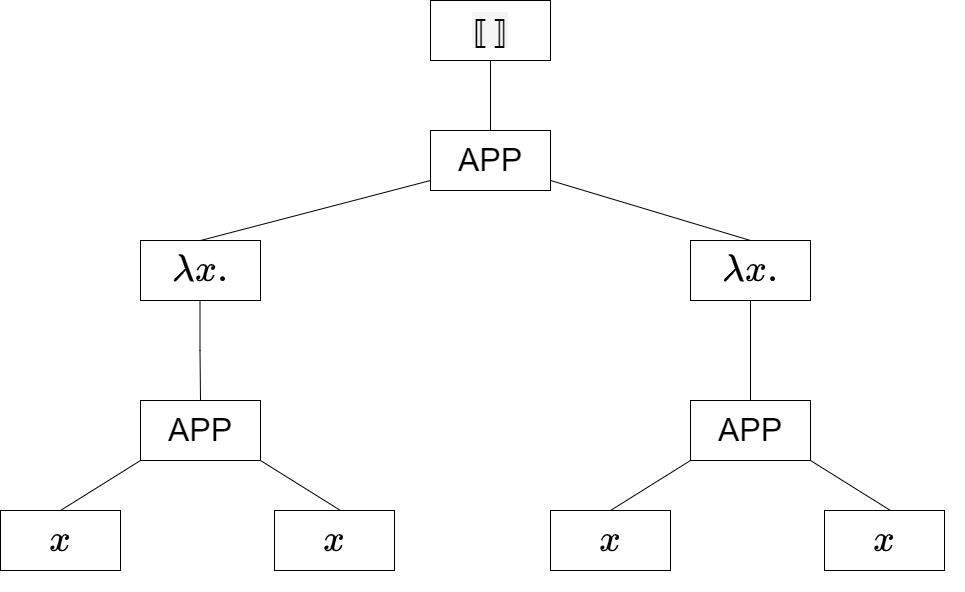
\includegraphics[width=\textwidth]{assets/ast_root_cursor.png}
  \end{minipage}\hfill
  \begin{minipage}{.45\textwidth}
    \center
    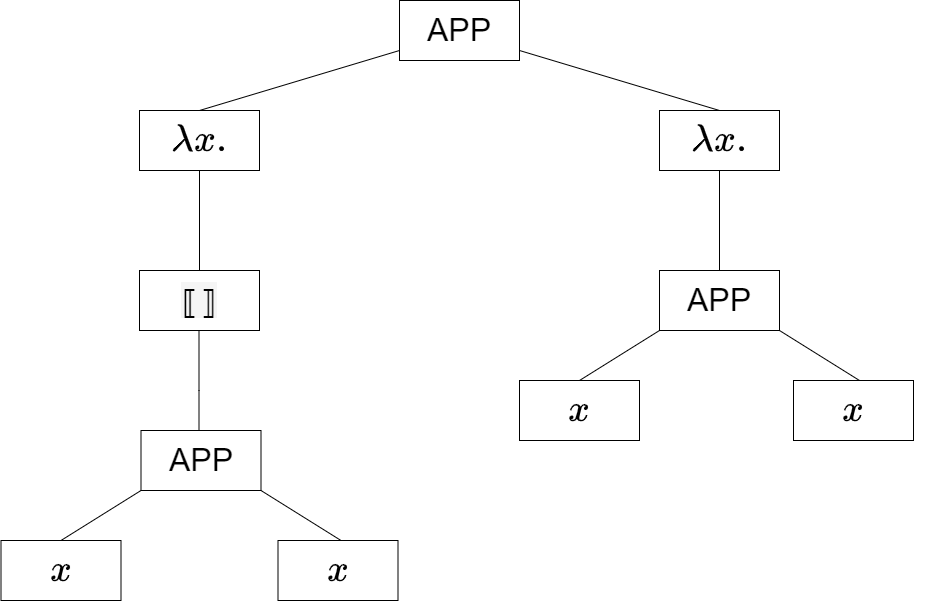
\includegraphics[width=\textwidth]{assets/ast_subtree_cursor.png}
  \end{minipage}\hfill
  \caption{An AST before and after cursor movement visualized in tree form}
  \label{fig:ast_visual_tree}
\end{figure*}

\subsection{Implementing a type checker}

Our editor typechecks configurations $\breakpoint{E,a}$. We say that
$\breakpoint{E,a}$ is well-typed iff both the AST $a$ is
well-formed and well-typed in the empty AST context and the editor
expression $E$
is both well-formed and well-typed for the path to the cursor in the AST and
the editor context containing all valid paths in the AST \pepm. This
is captured by the type rule
(\ref{eq:welltypedconf}) where $\emptyset$ is the empty AST context, $p$ is the
path from the root to the cursor in $a$, and $\ctx{e}$ is the editor context
containing some pair for each valid path in $a$.
%
\begin{equation}\label{eq:welltypedconf}
  \TConfiguration
\end{equation}
%
We have implemented the AST type rules using a function that pattern
matches on the given AST. E.g. for abstractions we follow the rule
\hyperref[fig:asttyperules]{(T-LAMBDA)} straightforwardly by judging
the type of its subtree and then wrapping it in the abstraction type,
remembering to add the binding to the context.

\begin{lstlisting}[language=elm,%
                    gobble=8,%
                    mathescape,%
                    ]
        Lambda x tau a_ ->
            Maybe.map (TLambda tau) <|
                typed a_ <| Ctx.bind x tau actx
\end{lstlisting}

Editor expression type judgements are a bit more involved. Since
editor expressions get their type information from an AST and not
themselves, we use Bool as return type rather than Maybe as we did for
AST rules. We require that the editor expression is completed. As we
did for AST type judgements, we pattern match on a given editor
expression and type check on a case by case basis.  E.g. regarding
substitution with abstractions, seen in the rule
\hyperref[fig:edttyperules]{(T-SUB-ABS)}, we first check if the path
$p$ is valid in the editor type context $\ctx{e}$. Then we find the
new context $\ctx{e}'$ by adding two new bindings to $\bar{p}$ and
check for consistency between the bound type and the type of the given
expression, and we recursively type check the next editor expression
$E$ in the new context $\ctx{e}'$.
\begin{lstlisting}[language=elm,%
                    gobble=8,%
                    mathescape,%
                    ]
        Pre (Aep.Sub (Aam.Lambda x tau1 tau2)) e ->
            case Ctx.get p ectx of
                Just (actx, atyp) -> let ectx_ =
                  Ctx.bind (Pth.extend p Ast.One)
                  (Ctx.bind x tau1 actx, tau2) <|
                    Ctx.bind p
                    (actx, Ast.TLambda tau1 tau2)
                      <| restrictBarPath p ectx
                  in
                  Ast.isConsistent atyp
                    (Ast.TLambda tau1 tau2)
                  && typed p ectx_ e
                Nothing -> False
\end{lstlisting}

\subsection{Building editor expressions}
Editor expressions written in a text field would have to be lexed and parsed.
This introduces syntax errors to the editor with regards to editor expressions,
which goes against the spirit of the editor. Hence we created a way to
build editor expressions in a similar manner to ASTs.

In order to build them, we need to introduce holes to the editor
expressions. We define a hole term constructor for each type of editor
expression, as seen in figure \ref{fig:editorexpressionswithholes}

\begin{figure}[H]
  \hspace{-6mm}
  \begin{tabular}{p{3.9cm}p{3.9cm}}
    \begin{lstlisting}[language=elm,%
                            gobble=8,%
                            mathescape,%
                            ]
             type Aep
                = Eval
                    $\vdots$
                | AepHole
        \end{lstlisting} &

    \begin{lstlisting}[language=elm,%
                            gobble=8,%
                            mathescape,%
                            ]
            type Eed
                = Neg Eed
                     $\vdots$
                | EedHole
        \end{lstlisting} \\

    \begin{lstlisting}[language=elm,%
                            gobble=8,%
                            mathescape,%
                            ]
            type Edt
                = Pre Aep Edt
                    $\vdots$
                | EdtHole
        \end{lstlisting} &

    \begin{lstlisting}[language=elm,%
                            gobble=8,%
                            mathescape,%
                            ]
            type Aam
                = Var Var.Id
                    $\vdots$
                | AamHole
        \end{lstlisting}
  \end{tabular}
  \caption{Editor expression definitions with holes}
  \label{fig:editorexpressionswithholes}
\end{figure}

We are now able to build editor expressions by initializing the editor
expression builder with an \texttt{EdtHole}, and then allow the user to
substitute holes with appropriate expressions. As with ASTs, we have the concept
of atomic editor expressions, which are editor expressions with holes as
children. The user can substitute holes until no holes are left. An editor
expression without any holes is said to be \textit{completed}.

We are only interested in evaluating completed editor expressions. To do this,
we introduce a type variable to each editor expression type. The type variable
is used for recursively defining the type in terms of the type variable, but
also as an argument to each hole constructor, as seen in the following
listing.

\begin{lstlisting}[language=elm,%
                   label="eed-definitions",%
                   gobble=4,%
                   ]
    type Eed a
        = Neg (Eed a)
        | Conjunction (Eed a) (Eed a)
        | Disjunction (Eed a) (Eed a)
        | At (Aam a)
        | Possibly (Aam a)
        | Necessarily (Aam a)
        | EedHole a
\end{lstlisting}

We utilize the \texttt{()} and the \texttt{Never} types to represent
completed and uncompleted editor expressions. If for example \texttt{a} in
\texttt{Edt a} is replaced with \texttt{()}, the editor expression can contain
holes. Conversely, if we replace \texttt{a} with \texttt{Never}, it cannot
contain holes, since we need a \texttt{Never} value to construct a hole. We can
therefore use \texttt{Edt ()} to represent uncompleted editor expressions, and
\texttt{Edt Never} to represent completed editor expressions. We have created a
type alias for completed and uncompleted editor expressions of every type.

This approach creates strong guarantees by making impossible states impossible.
The \texttt{toCompleted} function cannot take an \texttt{uncompleted} editor
expression, return a \texttt{completed} editor expression and still have bugs,
since we have constrained the types to create type level guarantees.

\subsection{The user interface}
\label{user-interface}

The user interface allows for two different visualizations of
programs: a textual representation and a tree representation. The
implementation of the textual representation is simple: A conversion
of the AST data structure to HTML with syntax highlighting . The last
image in figure \ref{fig:final_ui} shows this.

The implementation of the tree representation is more involved. Figure
\ref{fig:ast_visual_tree} shows an example of this

The visualization of the editor expression builder is similar to the textual
representation of ASTs. We implemented a function that given an \texttt{Edt}
returns HTML. An example of an
editor expression being built is in the upper left corner of the images in
figure \ref{fig:final_ui}.

\begin{figure*}
  \begin{center}
    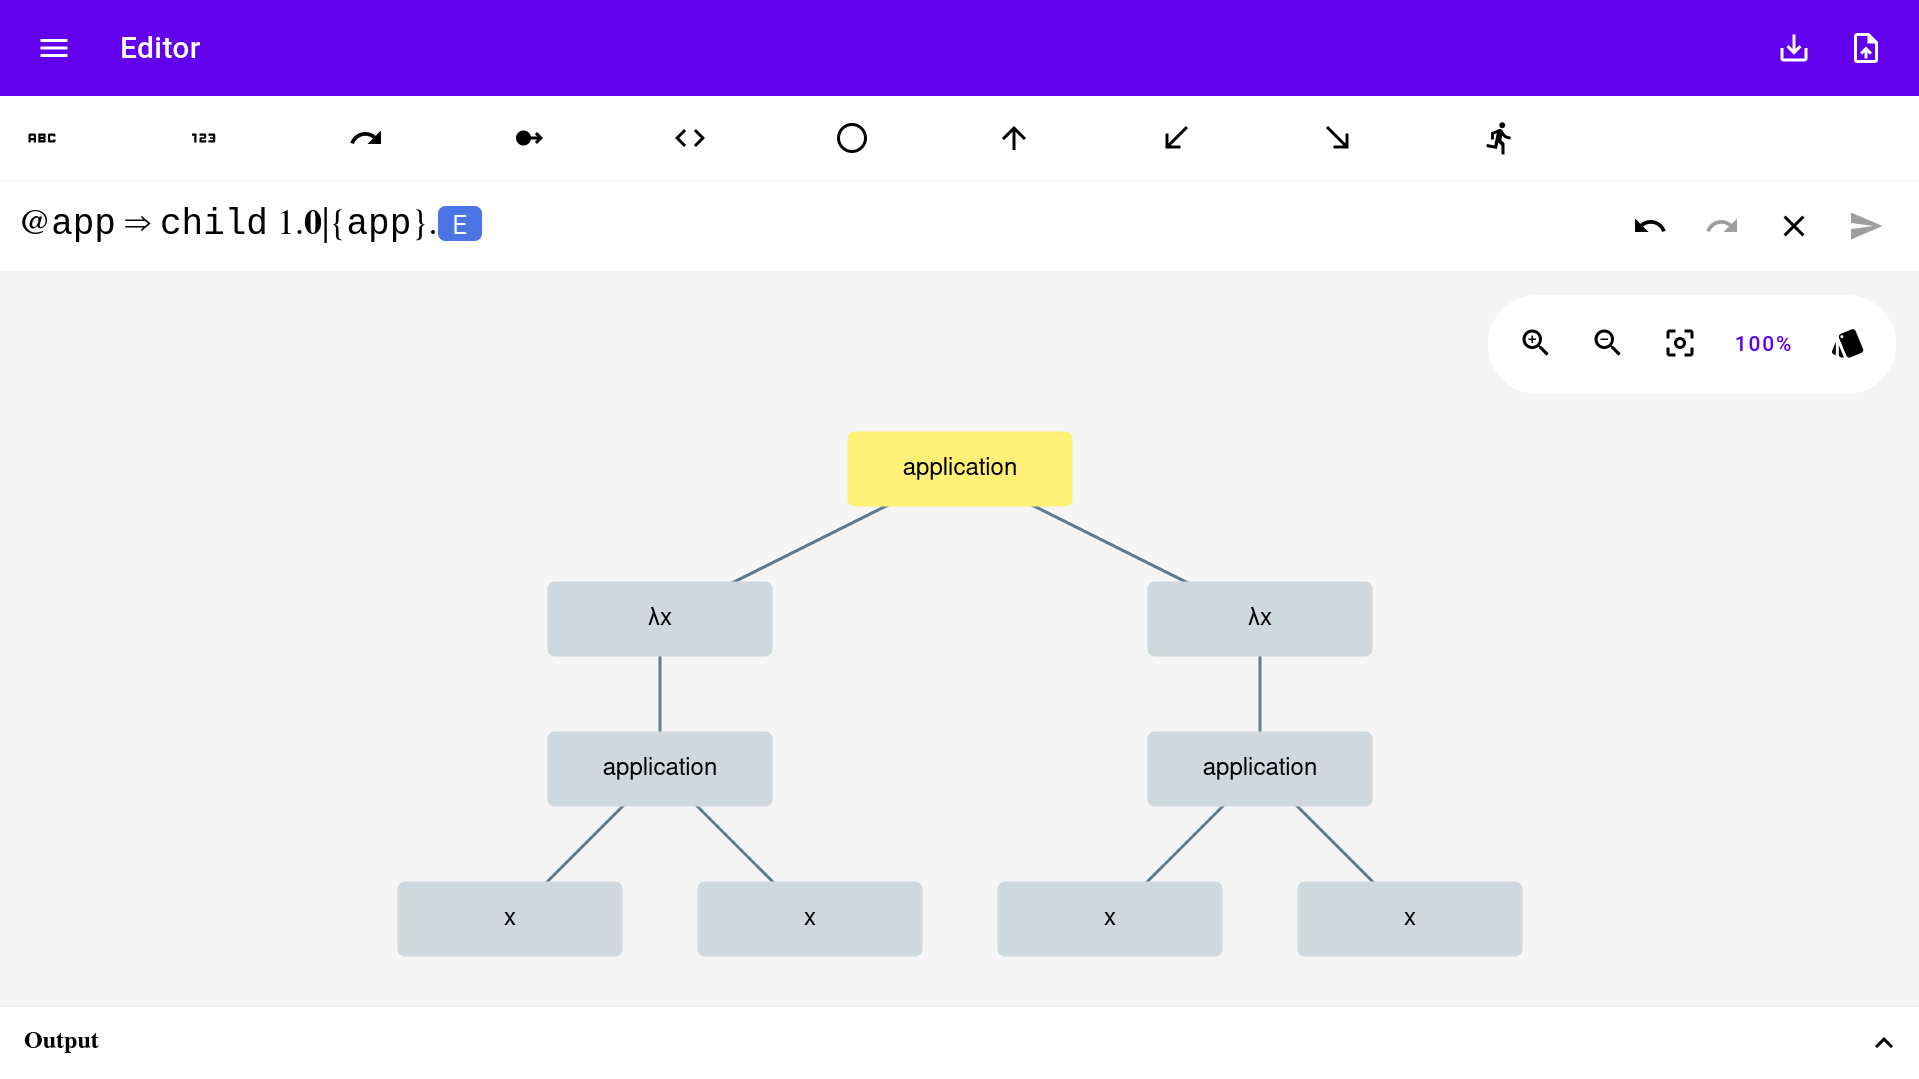
\includegraphics[width=0.7\textwidth]{assets/final_ui1.png}
  \end{center}
  \caption{A tree visualization}
  \label{fig:final_ui}
\end{figure*}

%%% Local Variables:
%%% mode: latex
%%% TeX-master: "../pepm2023"
%%% End:



\section{Conclusion}
\label{conclusion}

We have implemented the
editor calculus described by Godiksen et al. \pepm. The implementation
includes a tool for writing editor scripts and different
visualizations of abstract syntax trees that allows the user to move the view around and
zoom in and out of the tree visualization.

As programs get larger, one might want to collapse subtrees. This
comes with certain challenges for visualization. One problem is that if a subtree can be
collapsed, we likely want to ensure that the cursor is not in that
subtree, as the cursor would then be hidden. Similarly, if a subtree
is collapsed, the cursor should not be able to navigate into that
subtree.

One could attempt to evaluate the collapsed subtree and, if it
evaluates to a value, then show this as a summary.

Another feature that would improve usability is to make the default of the view
to follow the cursor when moving through the tree. There are a few different
ways to do it. The editor can follow the cursor with it being centered in the
view. Alternatively it can have the view follow whenever the cursor is near the
edge. For either of these cases, the editor could have a button that moves the
focus back to the cursor, making it possible to toggle between the locked and
the free view.


%%% Local Variables:
%%% mode: latex
%%% TeX-master: "../pepm2023"
%%% End:


%
% ---- Bibliography ----
%
% BibTeX users should specify bibliography style 'splncs04'.
% References will then be sorted and formatted in the correct style.
%

\bibliographystyle{ACM-Reference-Format}
\bibliography{references/references}



\end{document}

%%% Local Variables:
%%% mode: latex
%%% TeX-master: t
%%% End:
